\section{Mechanical meta-materials}
\label{sec:metamaterials}
Meta-materials are engineered materials with microstructure which results in macroscopic behavior not found in nature.
The most popularly known are electromagnetic meta-materials such as negative refraction index solids and ``invisibility cloaks'' which conceal an object through engineered distortion of electromagnetic fields \citep{poddubny2013hyperbolic,cai2010optical}.
However, they also hold great promise in other domains: \emph{mechanical} meta-materials use substructure to achieve unusual macroscopic behavior such as negative Poisson's ratio and nonlinear elastic responses; pores and lattices undergo reversible collapse under large deformation, enabling the engineering of complex physical affordances in soft robotics \citep{bertoldi2017flexible}.
\begin{wrapfigure}[12]{r}{0.4\textwidth}
\vspace{-0.2cm}
\centering
\begin{tabular}{c|c|c}
  		 {{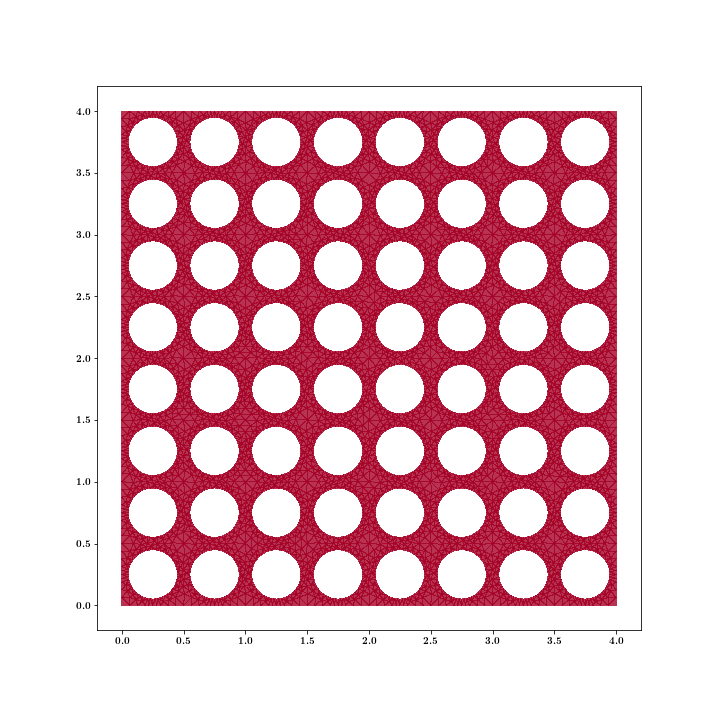
\includegraphics[height=1.1cm, trim={3.5cm 3.5cm 3.5cm 3.5cm}, clip]{lces/figures/rest_pore_0} }}&
  		{{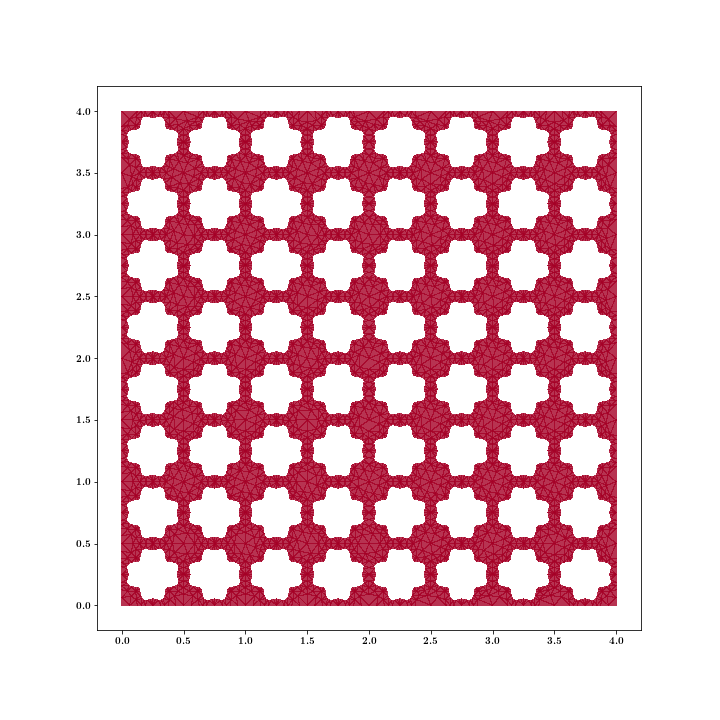
\includegraphics[height=1.1cm, trim={3.5cm 3.5cm 3.5cm 3.5cm}, clip]{lces/figures/rest_pore_01_-01} }}&%
  		{{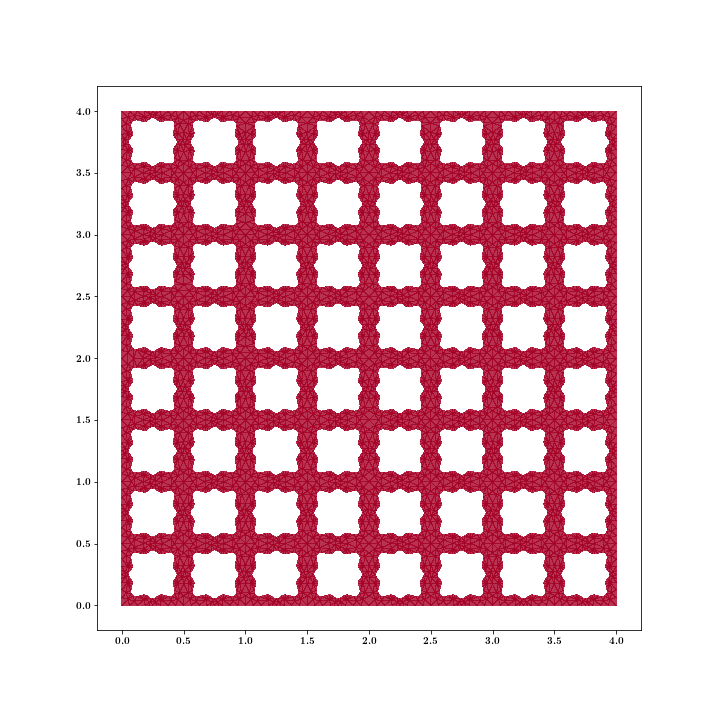
\includegraphics[height=1.1cm, trim={3.5cm 3.5cm 3.5cm 3.5cm}, clip]{lces/figures/rest_pore_-01_01} }}\\\hline
  	\rule{0pt}{7ex}
{{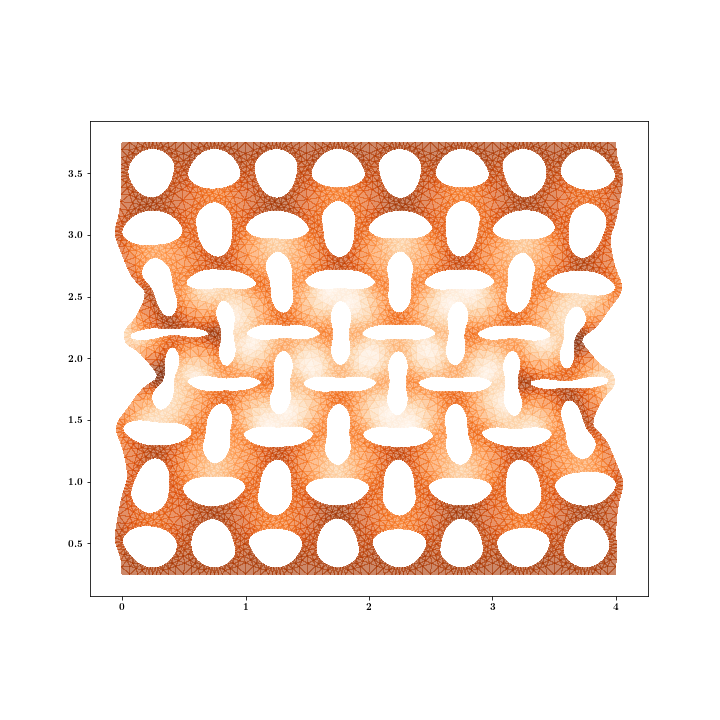
\includegraphics[height=0.95cm, trim={3.5cm 4.5cm 3.5cm 4.5cm}, clip]{lces/figures/pore_0} }}&%
  		{{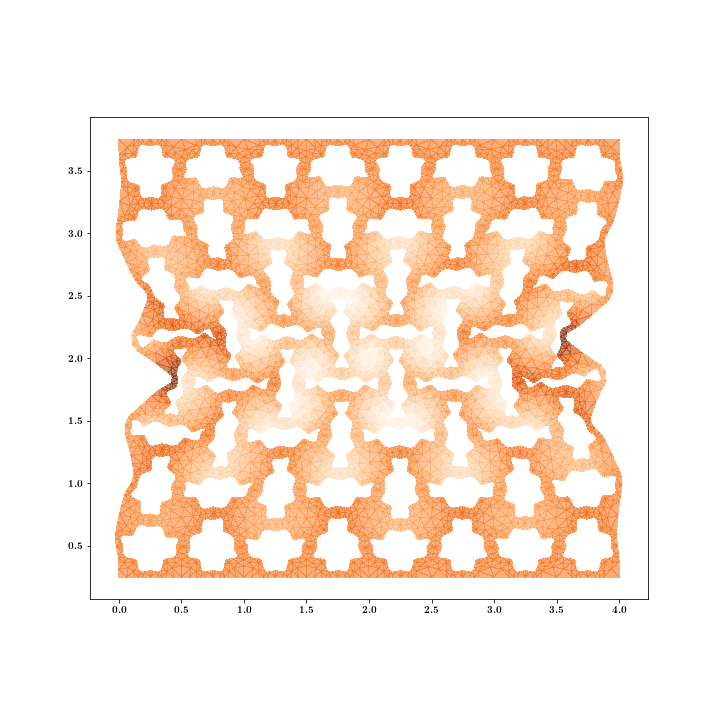
\includegraphics[height=0.95cm, trim={3.5cm 4.5cm 3.5cm 4.5cm}, clip]{lces/figures/pore_01_-01} }}&%
  		{{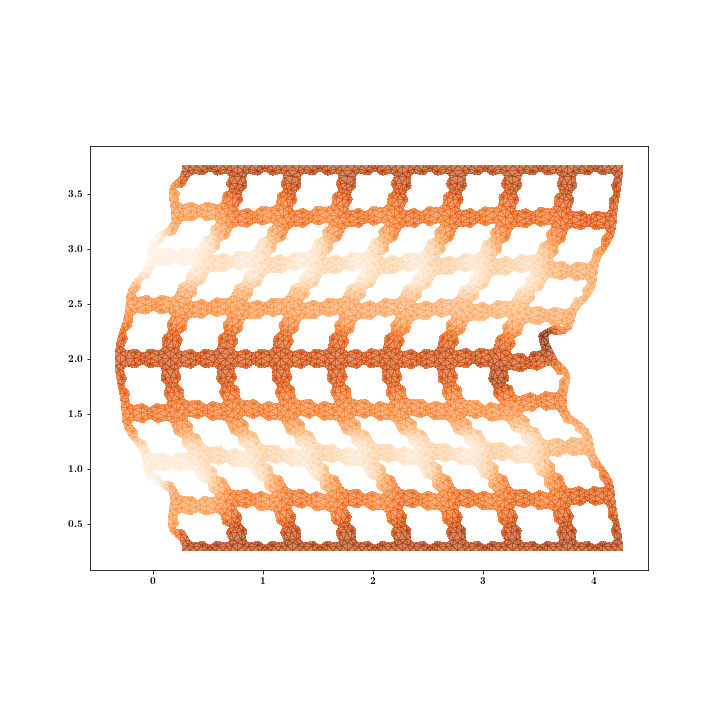
\includegraphics[height=0.9cm, trim={3.5cm 6cm 3.5cm 6cm}, clip]{lces/figures/pore_-01_01} }}%
  	\end{tabular}
  		\vspace{-0.2cm}%
  		\caption{\small Cellular meta-materials. Top: at rest. Bottom: under compression, exhibiting periodic instability varying with pore shape. The left two structures exhibit negative Poisson's ratio, which does not occur in nature.}%
  		\label{Fig:mms}%
\vspace{-0.4cm}
\end{wrapfigure}
Meta-materials hold promise for modern engineering design but are challenging to simulate as the microstructure necessitates a very fine finite element mesh, and as the nonlinear response makes them difficult to approximate with a macroscopic material model.
Most work on meta-materials has relied on engineers and scientists to hand-design materials, rather than numerically optimizing substructure to maximize some objective \citep{ion2016metamaterial}.

We focus on building surrogate models for the two-dimensional cellular solids investigated in \citet{overvelde2014relating}.
These meta-materials consist of square ``cells'' of elastomer, each of which has a pore in its center.
The pore shapes are defined by parameters~$\alpha$ and~$\beta$ which characterize the pore shape in polar coordinates:~${r(\theta) = r_0[1 + \alpha \cos(4\theta) + \beta \cos(8\theta)]}$.
The parameter $r_0$ is chosen such that the pore covers half the cell's volume:~${r_0 = \nicefrac{L_0}{\sqrt{\pi(2 + \alpha^2 + \beta^2}}}$. Constraints are placed on~$\alpha$ and~$\beta$ to enforce a minimum material thicknesses and ensure that $\min_\theta r(\theta) > 0$ as in \citet{overvelde2014relating}.

These pore shapes give rise to complicated nonlinear elastic behavior, including negative Poisson's ratio and double energy wells (i.e., stored elastic energy which does not increase monotonically with strain).
Realizations of this class of materials are shown under axial strain in Figure \ref{Fig:mms}. The continuum mechanics behavior of these elastomer meta-materials can be captured by a neo-Hookean energy model \citep{ogden1997non}.
Let~${X \in \mathbb{R}^d}$, where~${d\leq 3}$ in physical problems, be a point in the resting undeformed material reference configuration, and~$u(X)$ be the displacement of this point from reference configuration. The stored energy in a neo-Hookean solid is
%\begin{equation}
~${E = \int_{\Omega} W(u) dX\,,}$
%\end{equation}
where $W(u)$ is a scalar energy density over $\Omega$, defined for bulk and shear moduli~$\mu$ and~$\kappa$ as:
\begin{equation}\label{eq:neohookean}\small
   W = \frac{\mu}{2} \Big( (\det F)^{-2/d} \text{tr}(FF^T) - d\Big) + \frac{\kappa}{2} (\det F - 1)^2
\end{equation}
where $F$ is the deformation gradient,~${F(X) = \frac{\partial u(X)}{\partial X} + I\,.}$
Pores influence the structure of these equations by changing the material domain $\Omega$.
These solids can be simulated by solving:
\begin{equation}\label{eq:cm}\small
    \text{Div } S = 0 \quad X \in \Omega
\end{equation} \vspace{-0.4cm}
\begin{equation}\label{eq:bc}\small
    G(u) = 0 \quad X \in \partial \Omega
\end{equation}
where~${S = \frac{\partial W}{\partial F}}$ is known as the first Piola-Kirchoff stress, and where Eq.~\ref{eq:bc} defines a boundary condition.
E.g.~${G(u) = u - u_b}$ is a Dirichlet boundary condition; in our case, an externally imposed displacement. ${G(u) = \frac{\partial W}{\partial u} - f_b}$ corresponds to an external force exerting a pressure on the boundary.

To simulate these meta-materials, Eq.~\ref{eq:cm} is typically solved via finite element analysis.
Solving with large meta-material structures is computationally challenging due to fine mesh needed to capture pore geometry and due to the nonlinear response induced by buckling under large displacements.

Solving the PDE in Eq.~\ref{eq:cm} corresponds to finding the~$u$ which minimizes the stored energy in the material subject to boundary conditions.
That is, Eqs.~\ref{eq:cm} and~\ref{eq:bc} may be equivalently be expressed in an energy minimization form:
\begin{equation}\label{eq:cm-energy}\small
    		u = \argmin \int_{X \in \Omega}  W(u) dX \quad \quad\text{subject to } G(u) = 0 \in \partial\Omega
\end{equation}
We use this form to learn surrogates which solve the PDE in a reduced basis of cell boundaries.

\begin{wrapfigure}[12]{r}{0.28\linewidth}
\vspace{-1cm}
\centering
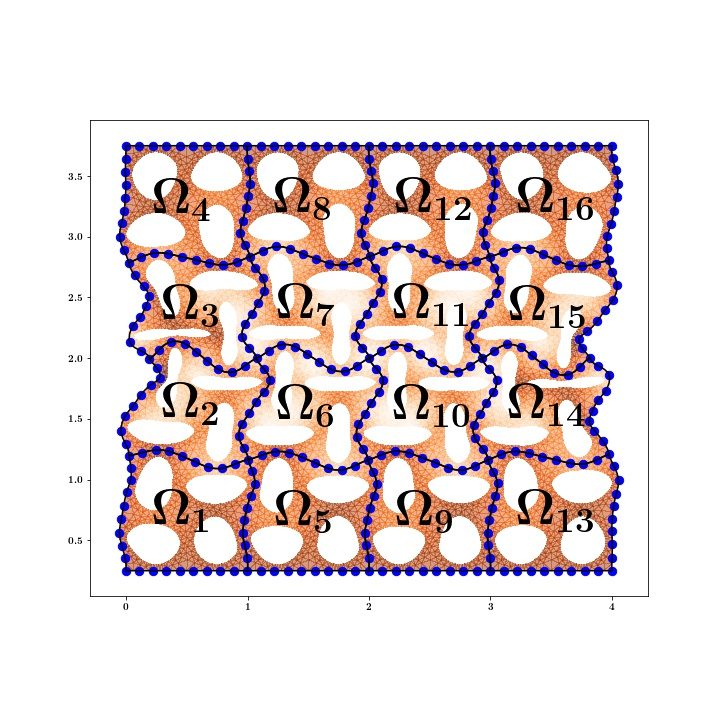
\includegraphics[height=2.7cm, trim={4.0cm 5cm 3.5cm 4.5cm}, clip]{lces/figures/decomp}
	\caption{\small Meta-material domain $\Omega$, partitioned into $\Omega_1$ to $\Omega_{16}$.
	Black lines show $\mathcal{B}$.
	Blue points are control points of splines used to represent $\tilde{u}$.\vspace{-.5cm}}
	\label{Fig:decomp}
\vspace{-.5cm}
\end{wrapfigure}
